\section{Game Abstraction Layer}


\begin{frame}
  \frametitle{GameAbstractionLayer klasse}

 	\begin{figure}
    	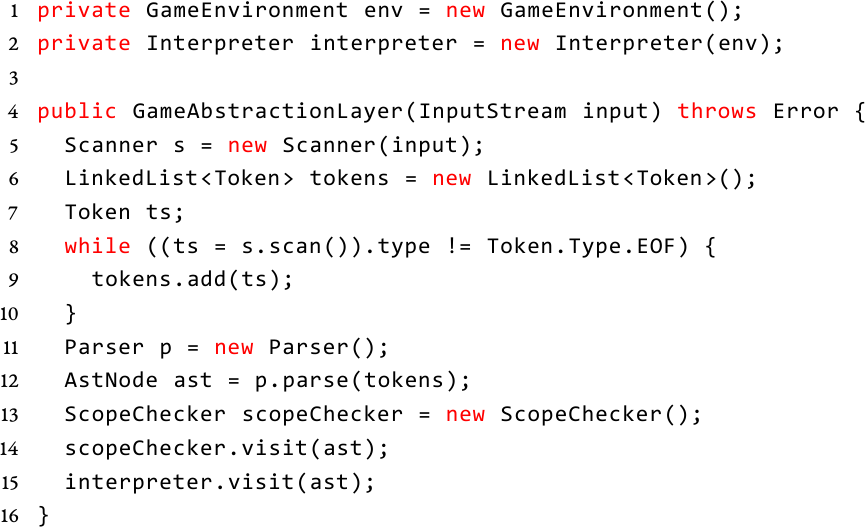
\includegraphics[width=0.8\linewidth]{billeder/gal_constructor_code.png}
 	\end{figure}
\end{frame}

\begin{frame}
  \frametitle{API}

  \begin{itemize}
    \item Et interface for hver type i Game Environment
    \item For hvert interface, en wrapper som implementerer det
  \end{itemize}
\end{frame}

\begin{frame}
  \frametitle{Game interface}

  \begin{tabular}{ c | c }
    Game & interface \\
    \hline
    players & getPlayers \\
    board & getBoard \\
    title & getTitle \\
    history & getHistory \\
    applyAction & applyAction \\
    nextTurn & nextTurn \\
     & getActions \\
  \end{tabular}
\end{frame}

\section{Simulator}

\begin{frame}
  \frametitle{Hensigt}

  \begin{itemize}
    \item Grafisk interface til GAL
	   \begin{itemize}
		  \item Skal kunne bruges af almindelige brugere
	   \end{itemize}
	 \item Gøre det let at teste og spille spil
  \end{itemize}
\end{frame}

\begin{frame}
  \frametitle{Widgets}

  \begin{itemize}
    \item Model til at styre input og visualisering
	 \item Organiseret i et hierarki
	 \item Indkapsler opførsel
  \end{itemize}
\end{frame}

\begin{frame}
  \frametitle{Widgets}

 	\begin{figure}
    	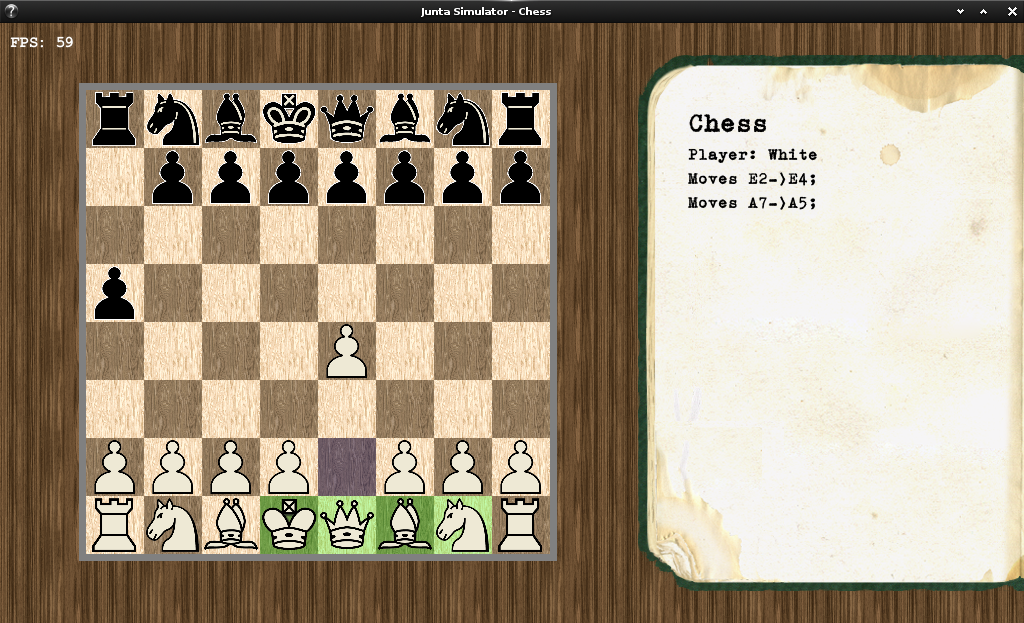
\includegraphics[width=0.8\linewidth]{billeder/simulator.png}
 	\end{figure}
\end{frame}

\begin{frame}
  \frametitle{Widgets}

 	\begin{figure}
    	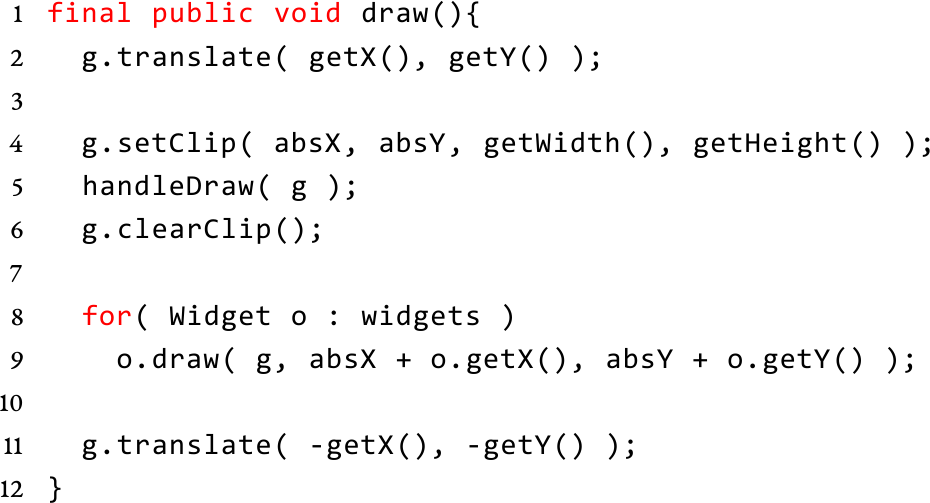
\includegraphics[width=0.8\linewidth]{billeder/widgets_draw_code.png}
 	\end{figure}
\end{frame}
